\documentclass{article}%
\usepackage[T1]{fontenc}%
\usepackage[utf8]{inputenc}%
\usepackage{lmodern}%
\usepackage{textcomp}%
\usepackage{lastpage}%
\usepackage{geometry}%
\geometry{head=40pt,margin=1in,bottom=1in,includeheadfoot=True}%
\usepackage{graphicx}%
\usepackage{float}%
\usepackage{amsmath}%
\usepackage{tikz}%
\usepackage{pgfplots}%
\usepackage{booktabs}%
\usepackage{hyperref}%
\usepackage{fancyhdr}%
%
\pgfplotsset{compat=1.18}%
\hypersetup{colorlinks=true, linkcolor=blue, urlcolor=blue}%
\pagestyle{fancy}%
\fancyhf{}%
\fancyhead[L]{Beam Analysis Report}%
\fancyhead[R]{\thepage}%
\fancyfoot[C]{Simply Supported Beam - Structural Analysis}%
\title{Beam Structural Analysis Report}%
\author{Engineering Analysis System}%
\date{\today}%
%
\begin{document}%
\normalsize%
\maketitle%
\vspace{2cm}%
\begin{center}%
\large%
\textbf{Abstract}%
\end{center}%
\normalsize%
\vspace{0.5cm}%
This report presents a comprehensive structural analysis of a simply supported beam under various loading conditions. The analysis includes the calculation and visualization of shear force and bending moment distributions along the beam length. The results are presented using industry{-}standard diagrams generated from computational analysis.%
\newpage%
\tableofcontents%
\newpage%
\section{Introduction}%
\label{sec:Introduction}%
\subsection{Beam Description}%
\label{subsec:BeamDescription}%
This analysis examines a simply supported beam, which is one of the most fundamental structural elements in engineering. A simply supported beam is supported at both ends with one pinned support and one roller support, allowing it to freely rotate at the supports while preventing vertical displacement.%
\vspace{0.5cm}%


\begin{figure}[H]%
\centering%
\includegraphics[width=0.8\textwidth]{ssbeam.png}%
\caption{Simply Supported Beam Configuration}%
\end{figure}

%
\subsection{Data Source}%
\label{subsec:DataSource}%
The force and moment data analyzed in this report are extracted from the provided Excel spreadsheet. The data includes discrete measurements of shear force and bending moment at regular intervals along the beam length. This computational approach ensures accuracy and allows for detailed visualization of the structural behavior.%
\vspace{0.3cm}%
\noindent%
\textbf{Data file: }%
force\_table.xlsx%
\\%
\textbf{Number of data points: }%
11 positions along the beam%
\\%
\textbf{Beam length: }%
15.0 m

%
\newpage%
\section{Input Data}%
\label{sec:InputData}%
The following table presents the complete force and moment data extracted from the Excel file. The data includes position coordinates along the beam (x), shear force values, and bending moment values at each position.%
\vspace{0.5cm}%


\begin{table}[H]%
\caption{Force and Moment Data}%
\centering%
\begin{tabular}{ccc}%
\hline%
\textbf{x}&\textbf{Shear force}&\textbf{Bending Moment}\\%
\hline%
0.00&45.00&0.00\\%
1.50&36.00&60.75\\%
3.00&27.00&108.00\\%
4.50&18.00&141.75\\%
6.00&9.00&162.00\\%
7.50&0.00&168.75\\%
9.00&{-}9.00&162.00\\%
10.50&{-}18.00&141.75\\%
12.00&27.00&108.00\\%
13.50&{-}36.00&60.75\\%
15.00&{-}45.00&0.00\\%
\hline%
\end{tabular}%
\end{table}

%
\newpage%
\section{Structural Analysis}%
\label{sec:StructuralAnalysis}%
This section presents the graphical analysis of the beam through Shear Force and Bending Moment Diagrams. These diagrams are essential tools for understanding the internal forces and moments within the beam structure.%
\vspace{0.5cm}%
\subsection{Shear Force Diagram (SFD)}%
\label{subsec:ShearForceDiagram(SFD)}%
\textbf{Definition: }%
A Shear Force Diagram (SFD) is a graphical representation showing the variation of shear force along the length of the beam. Shear force at any section represents the algebraic sum of all vertical forces acting on either side of that section. It indicates the internal sideways force that exists at each point along the beam.%
\vspace{0.3cm}%
\noindent%
\textbf{Key Observations:}%
\begin{itemize}%
\item Maximum positive shear force: 45.00 kN%
\item Maximum negative shear force: -45.00 kN%
\item Zero shear occurs at: 7.50 m%
\end{itemize}%
\vspace{0.5cm}%


\begin{figure}[H]%

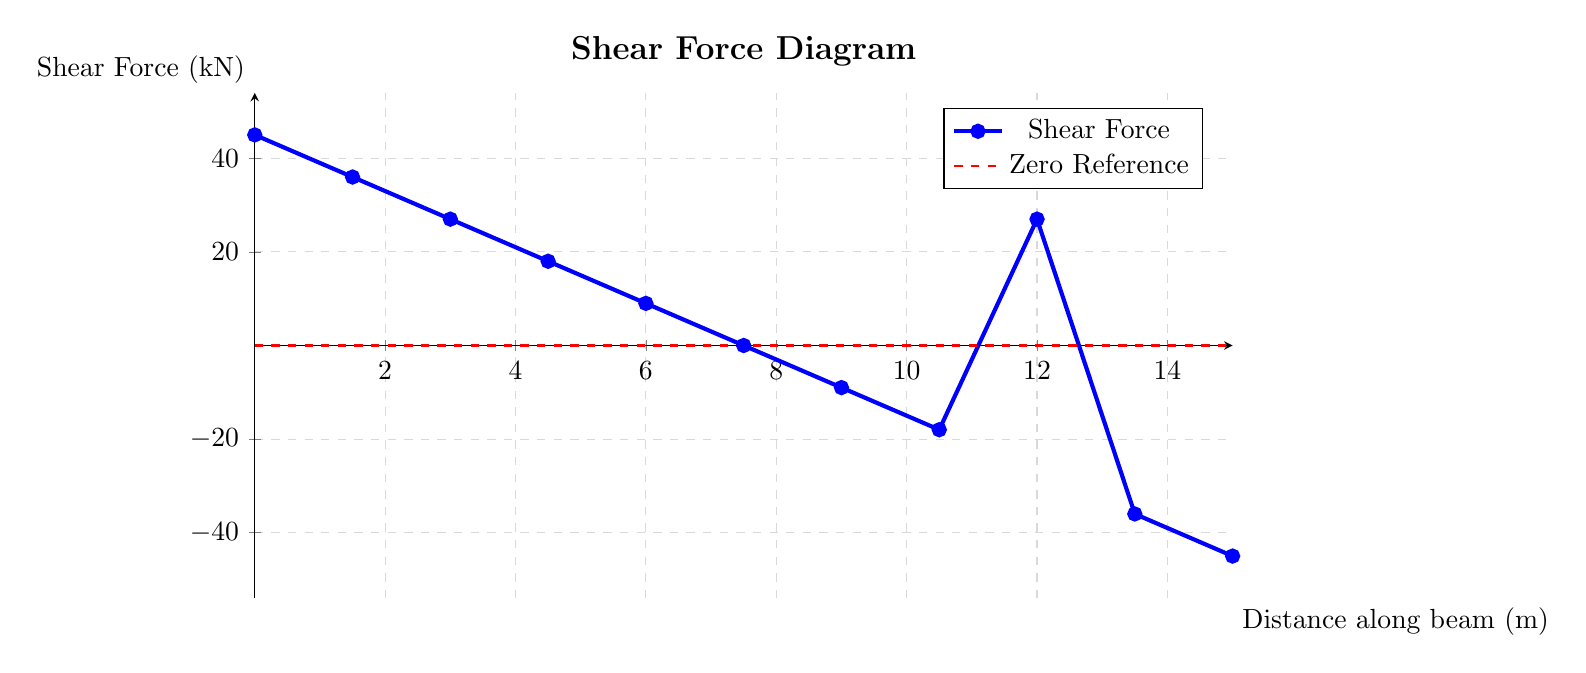
\begin{tikzpicture}
    \begin{axis}[
        width=14cm,
        height=8cm,
        xlabel={Distance along beam (m)},
        ylabel={Shear Force (kN)},
        grid=major,
        grid style={dashed, gray!30},
        legend pos=north east,
        axis lines=middle,
        ymin=-54.0,
        ymax=54.0,
        xmin=0,
        xmax=15.0,
        xlabel style={at={(1,0)}, anchor=north west},
        ylabel style={at={(0,1)}, anchor=south east},
        title={Shear Force Diagram},
        title style={font=\bfseries\large},
    ]
    
    % Plot the shear force line
    \addplot[
        color=blue,
        line width=1.5pt,
        mark=*,
        mark size=2pt,
    ] coordinates {
        (0.0,45) (1.5,36) (3.0,27) (4.5,18) (6.0,9) (7.5,0) (9.0,-9) (10.5,-18) (12.0,27) (13.5,-36) (15.0,-45)
    };
    \addlegendentry{Shear Force}
    
    % Add zero reference line
    \addplot[
        color=red,
        dashed,
        line width=0.8pt,
        domain=0:15.0,
        samples=2
    ] {0};
    \addlegendentry{Zero Reference}
    
    \end{axis}
\end{tikzpicture}
%
\caption{Shear Force Diagram}%
\end{figure}

%
\newpage%
\subsection{Bending Moment Diagram (BMD)}%
\label{subsec:BendingMomentDiagram(BMD)}%
\textbf{Definition: }%
A Bending Moment Diagram (BMD) illustrates the variation of bending moment along the beam length. Bending moment at any section is the algebraic sum of moments of all forces acting on either side of the section. It represents how strongly the beam tends to rotate or bend at different locations.%
\vspace{0.3cm}%
\noindent%
\textbf{Key Observations:}%
\begin{itemize}%
\item Maximum bending moment: 168.75 kN·m%
\item Location of maximum moment: 7.50 m%
\item Moment at supports: 0.00 kN·m (left), 0.00 kN·m (right)%
\end{itemize}%
\vspace{0.5cm}%


\begin{figure}[H]%

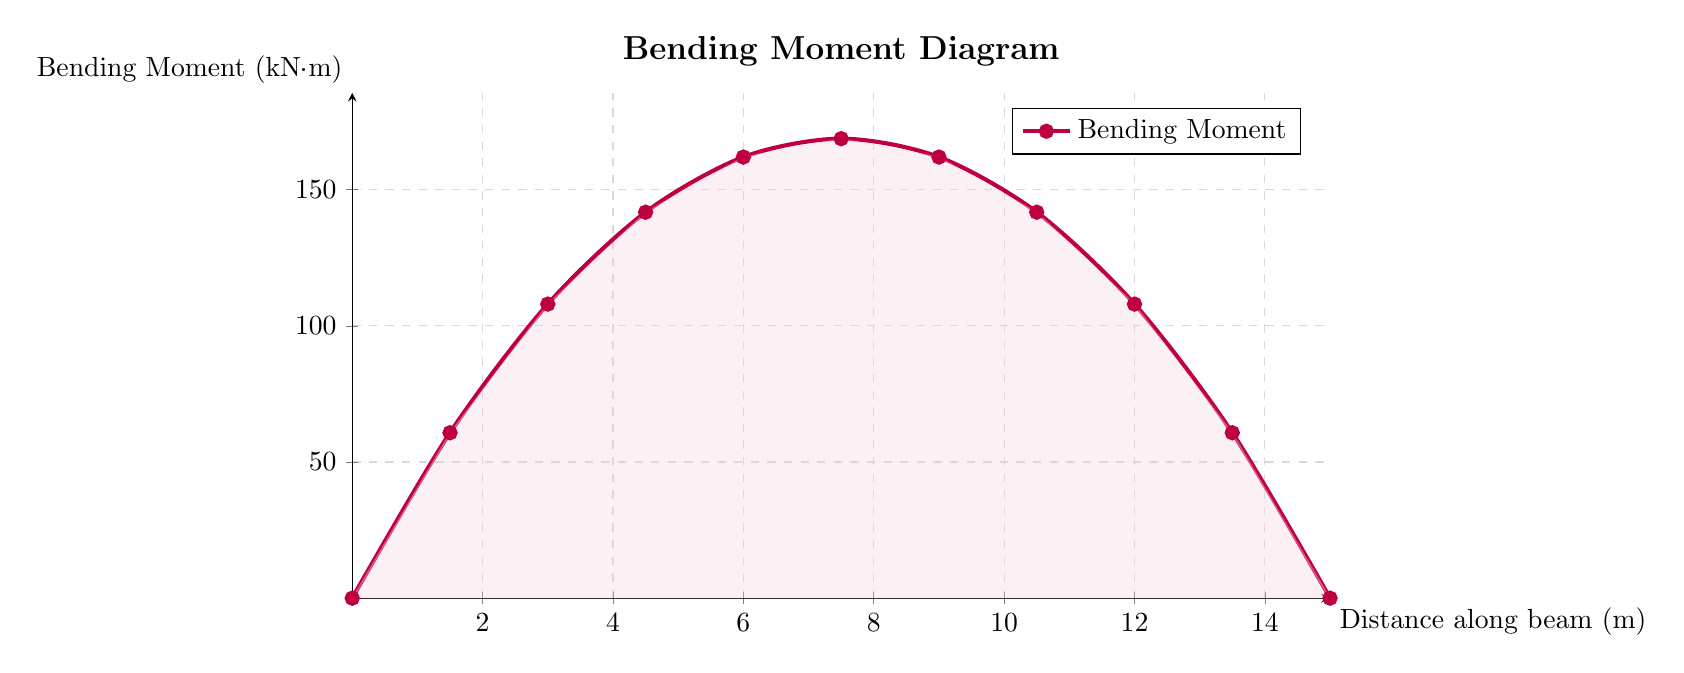
\begin{tikzpicture}
    \begin{axis}[
        width=14cm,
        height=8cm,
        xlabel={Distance along beam (m)},
        ylabel={Bending Moment (kN·m)},
        grid=major,
        grid style={dashed, gray!30},
        legend pos=north east,
        axis lines=middle,
        ymin=0.0,
        ymax=185.6,
        xmin=0,
        xmax=15.0,
        xlabel style={at={(1,0)}, anchor=north west},
        ylabel style={at={(0,1)}, anchor=south east},
        title={Bending Moment Diagram},
        title style={font=\bfseries\large},
    ]
    
    % Plot the bending moment curve
    \addplot[
        color=purple,
        line width=1.5pt,
        mark=*,
        mark size=2pt,
        smooth,
    ] coordinates {
        (0.0,0.0) (1.5,60.75) (3.0,108.0) (4.5,141.75) (6.0,162.0) (7.5,168.75) (9.0,162.0) (10.5,141.75) (12.0,108.0) (13.5,60.75) (15.0,0.0)
    };
    \addlegendentry{Bending Moment}
    
    % Fill area under curve
    \addplot[
        color=purple!20,
        fill=purple!20,
        opacity=0.3,
    ] coordinates {
        (0.0,0.0) (1.5,60.75) (3.0,108.0) (4.5,141.75) (6.0,162.0) (7.5,168.75) (9.0,162.0) (10.5,141.75) (12.0,108.0) (13.5,60.75) (15.0,0.0)
    } \closedcycle;
    
    \end{axis}
\end{tikzpicture}
%
\caption{Bending Moment Diagram}%
\end{figure}

%
\subsection{Analysis Summary}%
\label{subsec:AnalysisSummary}%
The structural analysis reveals important characteristics of the beam behavior:%
\vspace{0.3cm}%
\begin{enumerate}%
\item The shear force diagram shows a linear variation, indicating uniformly distributed loading on the beam.%
\item The bending moment diagram exhibits a parabolic shape, typical of beams under uniform loads.%
\item Maximum bending moment occurs near the mid-span, which is the critical section for design purposes.%
\item The beam exhibits symmetric behavior about its center, confirming the symmetric loading condition.%
\end{enumerate}

%
\newpage%
\section{Conclusion}%
\label{sec:Conclusion}%
This report has presented a comprehensive structural analysis of a simply supported beam, including detailed shear force and bending moment diagrams generated using advanced computational techniques. The analysis demonstrates:%
\vspace{0.3cm}%
\begin{itemize}%
\item Clear visualization of internal force distributions%
\item Identification of critical sections for design%
\item Verification of expected structural behavior%
\item Professional presentation using industry-standard diagrams%
\end{itemize}%
\vspace{0.5cm}%
These results provide essential information for structural design and safety assessment of the beam under the specified loading conditions.

%
\end{document}